% Section content template for individual Educative lessons
% This file contains the actual content for a specific section
% Generated from Educative API section content

% Section: System Design: Google Docs
% Section ID: 5540995072000000
% Section Slug: system-design-google-docs
% Generated: 2025-12-08T15:22:29.493883

\subsection{Problem statement}\label{gKGfVMqxnE595H2jISRuI}
\\
Imagine two students are preparing a report on a project they've just completed. Since the students live apart, the first student asks the second student to start writing the report, and the first student will improve the received copy. Although quite motivated, the students soon understand that such a collaboration is disorganized. The following illustration shows how tedious the process can get.

\begin{figure}[htbp]
 \centering
 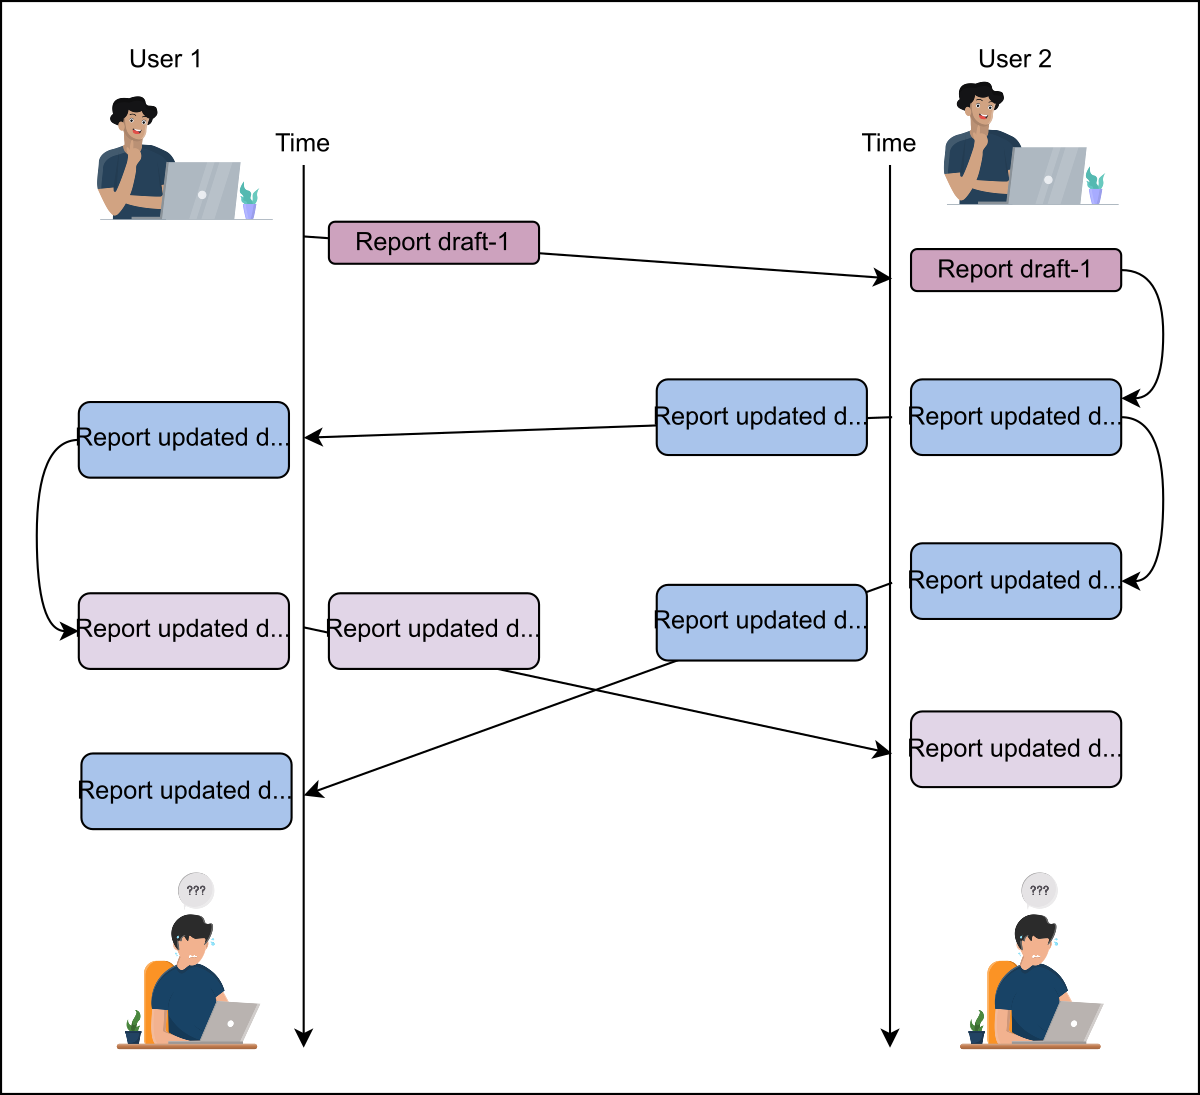
\includegraphics[width=0.5\textwidth]{Images/chapter_38/section_5540995072000000/4961336580898816.png}
 \caption{Problems arising when there’s no collaborative document editing service}
\end{figure}

The scenario above is one example that leads to time wastage and frustration when users collaborate on a document by exchanging files with each other.

\subsection{Google Docs}\label{NSH6Y4AN-cJvhosf0qSoZ}
\\
To combat the problem above, we can use an online collaborative document editing service like Google Docs. Some advantages of using an online document editing service instead of a desktop application are as follows:

\begin{itemize}
\item
\protect\phantomsection\label{d3Q9Pmla2M_ObA7vIU0v5}
Users can review and comment on a document while it's being edited.
\item
\protect\phantomsection\label{730d8KqnRgKsn92GdIWSl}
There are no special hardware specifications required to get the latest features. A machine that can run a browser will suffice.
\item
\protect\phantomsection\label{CJrH5HATwYs-AMcnlDcvR}
It\textquotesingle s possible to work from any location.
\item
\protect\phantomsection\label{g9XOGW6yU6-UVPxppN6Hz}
Unlike local desktop editors, users can view long-term document history and restore an older version if need be.
\item
\protect\phantomsection\label{TdN_T06JCUDusJkPZhipF}
The service is free of cost.
\end{itemize}
\\
Other than Google Docs, some popular online editing services include Etherpad, Microsoft Office 365, Slite, and many others.

\subsubsection{Designing Google Docs}\label{0VyYvoMaXs2q5ZXywH7ys}
\\
A collaborative document editing service can be designed in two ways:

\begin{itemize}
\item
\protect\phantomsection\label{HUDJbWh2AZR3MYmqWZkf7}
It could be designed as a centralized facility using client-server architecture to provide document editing service to all users.
\item
\protect\phantomsection\label{YK9iIZlTlRsKW5xt301Bo}
It could be designed using peer-to-peer technology to collaborate on a single document.
\end{itemize}

\begin{figure}[htbp]
 \centering
 
\includegraphics[width=0.15\textwidth]{Images/chapter_38/section_5540995072000000/4786703606611968.png}
 
\end{figure}

Most commercial solutions focus on client-service architecture to have finer control. Therefore, we'll focus on designing a service using the client service architecture. Let 's see how we will progress in this chapter.
\begin{quote}
\textbf{Note:} According to a survey(See: https://www.statista.com/forecasts/1011649/frequency-of-using-google-docs-in-the-us), 64\% of people use Google Docs for document editing at least once a week.
\end{quote}
\subsection{How will we design Google Docs?}\label{VS8HeKCLBqDA1YBS42VSY}
\\
We\textquotesingle ve divided the design problem into four stages:

\begin{enumerate}
\item
\protect\phantomsection\label{zuOBDl2YWx--66Q82GDiS}
\href{https://www.educative.io/courses/grokking-the-system-design-interview/requirements-of-google-docs-design}{\textbf{Requirements for Google Docs' Design}}: This lesson will focus on establishing the requirements for designing a collaborative document editing service. We'll also quantify the infrastructure requirements in this stage.
\item
\protect\phantomsection\label{wswurLJPJRgrdlr3ok7eq}
\href{https://www.educative.io/courses/grokking-the-system-design-interview/design-of-google-docs}{\textbf{Google Docs' Design}}: The goal of this lesson is to come up with a design that fulfills the requirements of the service. This lesson will explain why a component is used and how it integrates with other components to fulfill functional requirements.
\item
\protect\phantomsection\label{OmKSrU4R7uKdDf3vm3zTq}
\href{https://www.educative.io/courses/grokking-the-system-design-interview/concurrency-in-collaborative-editing}{\textbf{Concurrency in Collaborative Editing}}: Online document editing services have to resolve conflicts between users editing the same portion of a document. This lesson covers the type of problems that can arise and the techniques used to resolve such conflicts.
\item
\protect\phantomsection\label{wENc6TE5Uh9bOfZY0smf2}
\href{https://www.educative.io/courses/grokking-the-system-design-interview/evaluation-of-google-docs-design}{\textbf{Evaluating Google Docs' Design}}: The main objective of this lesson is to evaluate our design for non-functional requirements. Mainly, we see if our design is performant, consistent, available, and scalable.
\end{enumerate}
\\
If you want to get hands-on experience with how to build a simple collaborative document editing system in AWS, consider exploring the following AWS Cloud Lab.

Let's begin with a look at our requirements.

% End of section content